% Alphabet = set of nucleotides: 
% A,C,G,T
\newcommand{\cga}{{\color{red!70!black} A}}
\newcommand{\cgc}{{\color{blue!70!black} C}}
\newcommand{\cgg}{{\color{yellow!70!black} G}}
\newcommand{\cgt}{{\color{green!70!black} T}}


\begin{frame}{Sequence processing}
  \begin{block}{Sequence generation model}
    $$
    P(\wsseq{1}{L}) = P(\ws_1, \ws_2, ... \ws_L) = \prod_{i=1}^L P(\ws_i | \wsseq{1}{i-1}),\ \ \forall i , \ws_i \in \vocab
    $$
    with the \textbf{\ngram assumption} (convolution):
    $$
    P(\wsseq{1}{L}) = \prod_{i=1}^L P(\ws_i | \wsseq{i-n+1}{i-1}),\ \ \forall i , \ws_i \in \vocab,
    $$
    in the \textbf{recurrent} way 
    $$ P(\ws_i | \wsseq{1}{i-1})$$
  \end{block}
  \begin{block}{Sequence representation}
    \begin{center}
      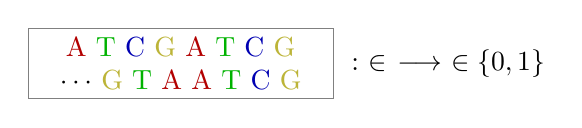
\begin{tikzpicture}
        %%%%%%%%%%%%%%%%%%%%% 
        \node[anchor=east,draw=gray,text width=0.3\textwidth,align=center] (review) at
        (0,0) {\cga~\cgt~\cgc~\cgg~\cga~\cgt~\cgc~\cgg\\$\cdots$~\cgg~\cgt~\cga~\cga~\cgt~\cgc~\cgg};
        %%%%%%%%%%%%%%%%%%%%% 
        \node[anchor=west] (txt) at (0.1,0) {$: \ \x \in \real^{\nfeats} \ \longrightarrow \ \class \in\{0, 1\}$};
      \end{tikzpicture}
    \end{center}
  \end{block}
\end{frame}

